\section{Diagramma Componenti}

\subsection{Diagramma dei Componenti}
\begin{figure}[H]
    \centering
    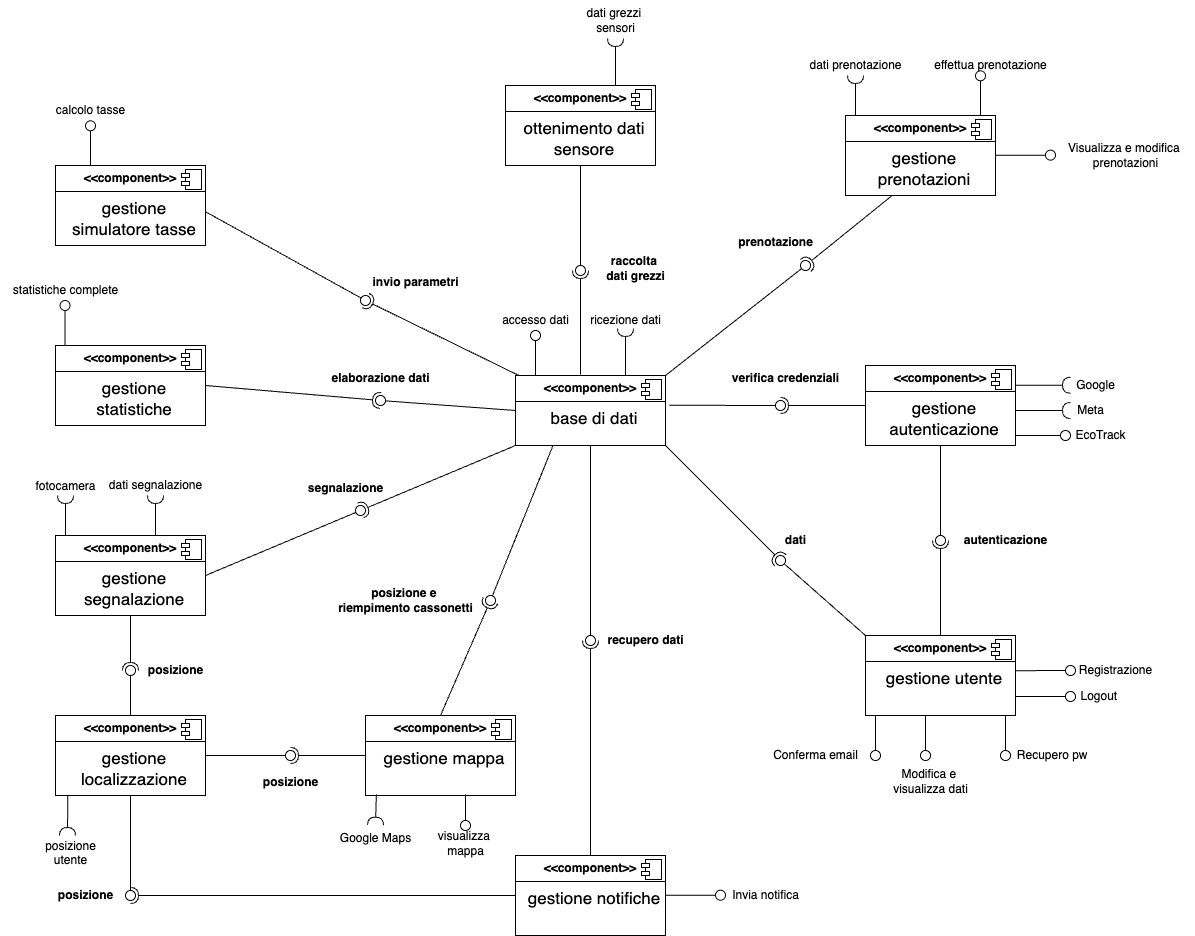
\includegraphics[width=1\linewidth]{D2-G1//Img/Component Diagram.png}
    \caption{Diagramma dei componenti}
    \label{fig:enter-label}
\end{figure}

\subsection{Descrizione dei Componenti}

\subsubsection{Gestione Autenticazione}  
Il componente gestisce l'autenticazione dell'utente, la quale può essere effettuata in diversi modi.

\begin{table}[H]
    \centering
    \begin{tabular}{|c|c|p{9cm}|}
        \hline
        \textbf{Tipologia} & \textbf{Nome} & \textbf{Descrizione} \\
        \hline
        Richiesta & Google & Il componente utilizza un’interfaccia fornita da Google per autenticarsi tramite un token (SSO) \\
        \hline
        Richiesta & Meta & Il componente utilizza un’interfaccia fornita da Meta per autenticarsi tramite un token (SSO) \\
        \hline
        Fornita & EcoTrack & Il componente fornisce un'interfaccia per autenticarsi mediante gli account locali \\
        \hline
        Fornita & Autenticazione & Il componente fornisce un'interfaccia per autenticarsi \\
        \hline
        Richiesta & Verifica credenziali & Il componente richiede che le credenziali vengano verificate \\
        \hline
    \end{tabular}
    \caption{Componenti coinvolti nella gestione dell'autenticazione}
    \label{tab:gestione_autenticazione}
\end{table}

\subsubsection{Gestione Localizzazione}  
Questo componente gestisce le interazioni con il sistema di localizzazione (GPS).

\begin{table}[H]
    \centering
    \begin{tabular}{|c|c|p{9cm}|}
        \hline
        \textbf{Tipologia} & \textbf{Nome} & \textbf{Descrizione} \\
        \hline
        Fornita & Posizione & Il componente fornisce (in coordinate) la posizione attuale dell'utente \\
        \hline
        Richiesta & Posizione utente & Il componente richiede la posizione attuale dell'utente \\
        \hline
    \end{tabular}
    \caption{Componenti coinvolti nella gestione della localizzazione}
    \label{tab:gestione_localizzazione}
\end{table}

\subsubsection{Base di Dati}  
Questo componente gestisce tutti i dati coinvolti nel funzionamento dell'applicazione e permette agli altri componenti di relazionarsi.

\begin{table}[H]
    \centering
    \begin{tabular}{|c|c|p{9cm}|}
        \hline
        \textbf{Tipologia} & \textbf{Nome} & \textbf{Descrizione} \\
        \hline
        Fornito & Verifica credenziali & Il componente effettua la verifica delle credenziali utilizzate \\
        \hline
        Fornito & Prenotazione & Il componente verifica gli orari disponibili e salva una prenotazione \\
        \hline
        Richiesto & Raccolta dati grezzi & Il componente raccoglie i dati grezzi direttamente dai sensori \\
        \hline
        Richiesto & Invio parametri & Il componente salva i parametri relativi al simulatore tasse \\
        \hline
        Fornito & Elaborazione dati & Il componente fornisce i dati grezzi, che devono essere elaborati. In seguito, i dati elaborati verranno inviati al componente in questione. \\
        \hline
        Richiesto & Segnalazione & Il componente salva un'eventuale segnalazione e mostra le segnalazioni già salvate \\
        \hline
        Fornito & Posizione e riempimento cassonetti & Il componente fornisce la posizione (coordinate) e il livello di riempimento dei cassonetti \\
        \hline
        Fornito & Recupero dati & Il componente fornisce i dati che potrebbero far scaturire una notifica \\
        \hline
        Richiesto & Dati & Il componente richiede e mostra i dati relativi ai vari utenti \\
        \hline
    \end{tabular}
    \caption{Componenti coinvolti nella gestione della base di dati}
    \label{tab:base_dati}
\end{table}
